% \meutodo{
%   Experimentos:
%   - Descrição das bases
%   - Descrição das ferramentas/técnicas/pacotes
%   - Descrição do protocolo
%   - Apresentação dos resultados
%   - Discussão dos resultados
% }
%
% \meutodo{
%   Variação gradual de parâmetros para identificar o que causa perdas/ganhos
% }

%%%%%%%%%%%%%%%%%%%%%%%%%%%%%%%%%%%%%%%%%%%%%%%%%%%%%%%%%%%%%%%%%%%%%%%%%%%%%%%%
\section{Considerações Iniciais}


%%%%%%%%%%%%%%%%%%%%%%%%%%%%%%%%%%%%%%%%%%%%%%%%%%%%%%%%%%%%%%%%%%%%%%%%%%%%%%%%
\section{Quantização de Imagens}

Diferentes métodos de quantização produzem diferentes resultados em termos de acurácia. Quando comparado com métodos mais complexos, esse procedimento permite uma redução de dimensionalidade significante, enquanto preserva ou melhora a acurácia do sistema.

\begin{figure}[htbp]
  \begin{center}
    \centering
    \includegraphics[width=0.4\linewidth]{\detokenize{figuras/quantizacao/quantizationResult.png}}
  \end{center}
\end{figure}

%%%%%%%%%%%%%%%%%%%%%%%%%%%%%%%%%%%%%%%%%%%%%%%%%%%%%%%%%%%%%%%%%%%%%%%%%%%%%%%%
\subsection{Base de Imagens}

%%%%%%%%%%%%%%%%%%%%%%%%%%%%%%%%%%%%%%%%%%%%%%%%%%%%%%%%%%%%%%%%%%%%%%%%%%%%%%%%
\subsection{Protocolo}



%%%%%%%%%%%%%%%%%%%%%%%%%%%%%%%%%%%%%%%%%%%%%%%%%%%%%%%%%%%%%%%%%%%%%%%%%%%%%%%%
\subsection{Resultados e Discussão}




%%%%%%%%%%%%%%%%%%%%%%%%%%%%%%%%%%%%%%%%%%%%%%%%%%%%%%%%%%%%%%%%%%%%%%%%%%%%%%%%
\section{Geração de Imagens Artificiais}

Essa seção descreve os resultados encontrados ao rebalancear as classes de imagens. Na figura \ref{fig:fluxo} é possível observar o fluxo de operações realizadas para analisar o impacto da geração de imagens no rebalanceamento de classes. O mesmo protocolo de conversão para escala de cinza, extração de características e classificação foi seguido para três experimentos: base desbalanceada; base rebalanceada com interpolação dos vetores de características; e base rebalanceada com a geração artificial de imagens. Portanto inicia-se com a descrição destas bases de imagens, a descrição do protocolo adotado e por fim os resultados obtidos a partir de seu uso são mostrados e discutidos.

\begin{figure}[thpb]
\centering
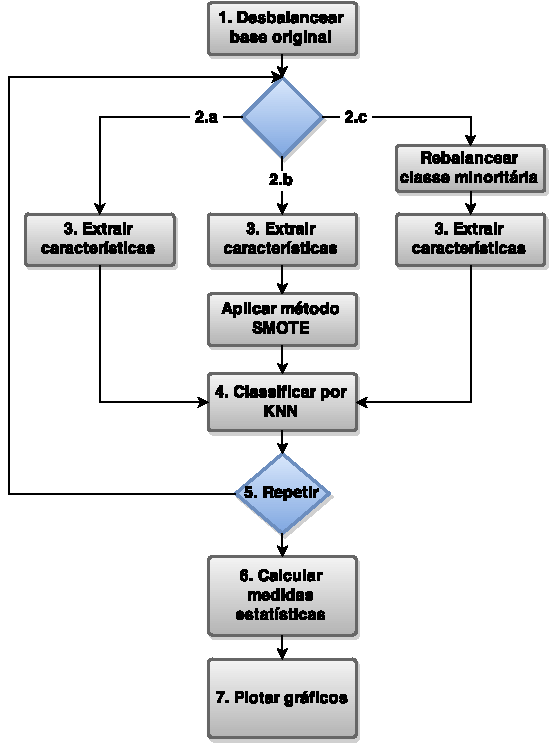
\includegraphics[scale=0.8]{\detokenize{figuras/flow_main.pdf}}
\caption{Fluxo de operações do experimento realizado.}
\label{fig:fluxo}
\end{figure}


%%%%%%%%%%%%%%%%%%%%%%%%%%%%%%%%%%%%%%%%%%%%%%%%%%%%%%%%%%%%%%%%%%%%%%%%%%%%%%%%
\subsection{Base de Imagens}

 Os resultados foram obtidos utilizando a base de imagens COREL\footnote{Disponível em http://wang.ist.psu.edu/docs/related/}, composta por fotografias que representam classes variadas: tribos africanas, praia, construções, ônibus, dinossauros, elefantes, flores, cavalos, montanhas e tipos de comidas. São 10 classes balanceadas com 100 imagens cada. Para fins de exemplificação, são apresentadas amostras das imagens que representam essas classes na Figura \ref{fig:corel}.

 \begin{figure}[hbpt]
 \begin{center}
   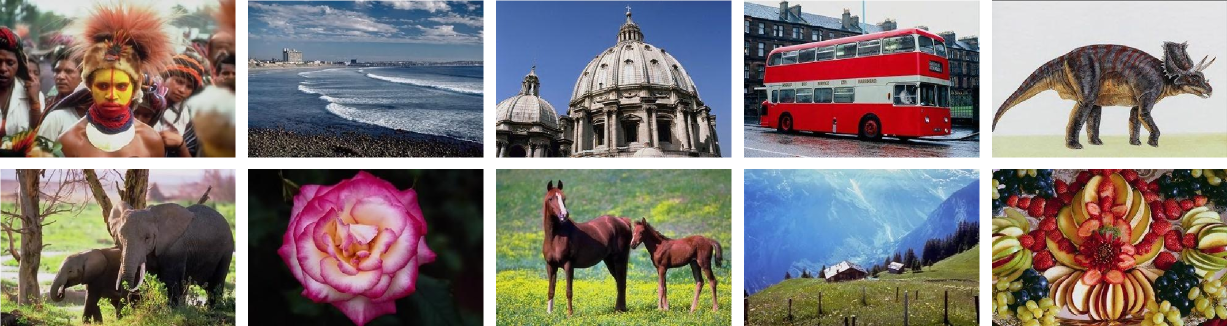
\includegraphics[width=1\linewidth]{\detokenize {figuras/exemplos_corel.png}}
 \end{center}
  \caption[Base de imagens COREL-1000.]{Base de imagens COREL-1000 utilizada. Estão representadas as 10 classes da base. \textit{Fonte: Elaborado pela autora.}}
 \label{fig:corel}
\end{figure}

%%%%%%%%%%%%%%%%%%%%%%%%%%%%%%%%%%%%%%%%%%%%%%%%%%%%%%%%%%%%%%%%%%%%%%%%%%%%%%%%
\subsection{Protocolo}

O seguinte protocolo foi seguido para a obtenção dos resultados:

\begin{enumerate}
\item \textbf{Classes de imagens originais}: classes Elefante e Cavalo da COREL-1000;
\item \textbf{Amostragem dos dados}: 50\% para treino e 50\% para teste de cada classe;
\item \textbf{Desbalanceamento}: remoção de 50\% do conjunto de treino da classe Cavalo;
\item \textbf{Método para geração artificial}: mistura de duas imagens originais, exemplificado na Figura~\ref{fig:mistura};
\item \textbf{Quantização}: Intensidade. É o método mais simples de converter uma imagem colorida em tons de cinza. Consiste em computar a média entre os canais RGB da imagem a partir de
\begin{equation}
	Q_{Intensidade} = \frac{1}{3}(R + G + B)
\end{equation}
\noindent e então realizar uma correção por \textit{gamma};
\item \textbf{Extração de características}: classificação de pixels de borda e interior (BIC). Computa dois histogramas, um para pixels definidos como borda e outro como interior. Se um pixel possuir a mesma cor que seus vizinhos, é considerado pixel de interior; caso contrário, será pixel de borda. Os histogramas são concatenados em um vetor de $2N$ dimensões, onde $N$ é o número de intensidades de cor da imagem \cite{bic};
\item \textbf{Classificação}: classificador supervisionado K=NN com $K = 1$ (para mais detalhes ver Seção~\ref{sec:knn});
\item \textbf{Projeção multidimensional}: projetados os dois componentes principais encontrados ao aplicar PCA nos vetores de características para redução de dimensionalidade (Seção~\ref{sec:pca}). A implementação desenvolvida para esta projeção pode ser encontrada em \url{https://github.com/GabiThume/msc-src/blob/master/visualization/plot.py}. Vale destacar que uma animação da adição de cada novo exemplo foi realizada para fim de visualizar o melhor subespaço gerado.
\end{enumerate}
%%%%%%%%%%%%%%%%%%%%%%%%%%%%%%%%%%%%%%%%%%%%%%%%%%%%%%%%%%%%%%%%%%%%%%%%%%%%%%%%
\subsection{Resultados e Discussão}

As classes Elefante e Cavalo possuem 100 imagens cada. O primeiro passo é remover imagens de uma das classes, tornando a base desbalanceada. Como o foco é na visualização do espaço de características, é relevante ter o modelo do espaço ideal das classes balanceadas, por isso esse experimento em específico não trata de uma base naturalmente desbalanceada. Na Figura~\ref{fig:desbalanceado} está ilustrada a remoção de 50\% das imagens de treino da classe Cavalo, originalmente balanceada. Essa e as próximas projeções desta seção foram obtidas com a técnica para redução de dimensionalidade PCA, descrita na Seção~\ref{sec:pca} e são referentes aos dois componentes principais com maiores autovalores.

\begin{figure}[htbp]
  \begin{center}
    \begin{subfigure}{.49\linewidth}
      \centering
      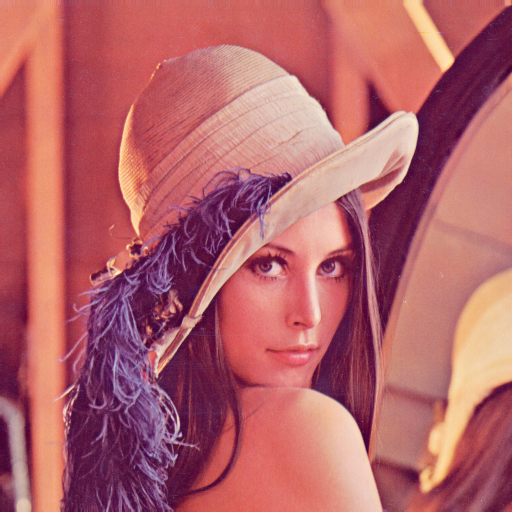
\includegraphics[width=\linewidth]{\detokenize{figuras/visualizacao/original.png}}
    \end{subfigure}
    \begin{subfigure}{.49\linewidth}
      \centering
      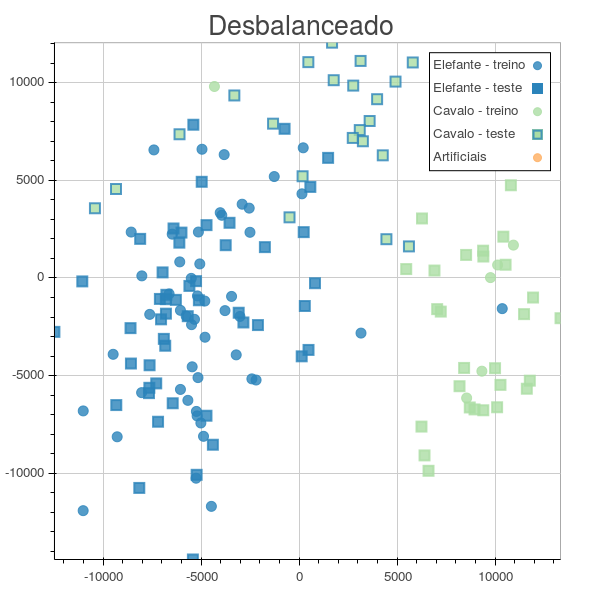
\includegraphics[width=\linewidth]{\detokenize{figuras/visualizacao/desbalanceado-fixed.png}}
    \end{subfigure}
  \end{center}
  \caption{Remoção de 50\% das imagens de treino da classe Cavalo.}
  \label{fig:desbalanceado}
\end{figure}

A classificação dos três experimentos utilizando KNN reportou que o \textit{f-score} da geração artificial de imagens utilizando o método de mistura teve um ganho de mais de 10\% em relação ao rebalanceamento no espaço de características com o SMOTE. Para confirmar que a geração aqui proposta inseriu mais informação na classe minoritária do que apenas povoar os espaços entre os exemplos (i.e.\ SMOTE), a classe rebalanceada utilizando ambos métodos está demonstrada na Figura~\ref{fig:compara_vis_treino_fixed}. Em laranja estão representados os novos exemplos de treinamento, projetados no plano da base original balanceada.

\begin{figure}[htbp]
  \begin{center}
    \begin{subfigure}{.49\linewidth}
      \centering
      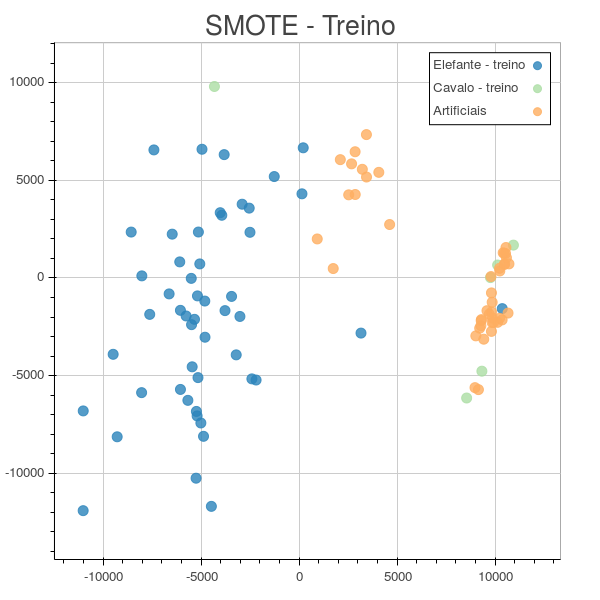
\includegraphics[width=\linewidth]{\detokenize{figuras/visualizacao/smote-treino-fixed.png}}
    \end{subfigure}
    \begin{subfigure}{.49\linewidth}
      \centering
      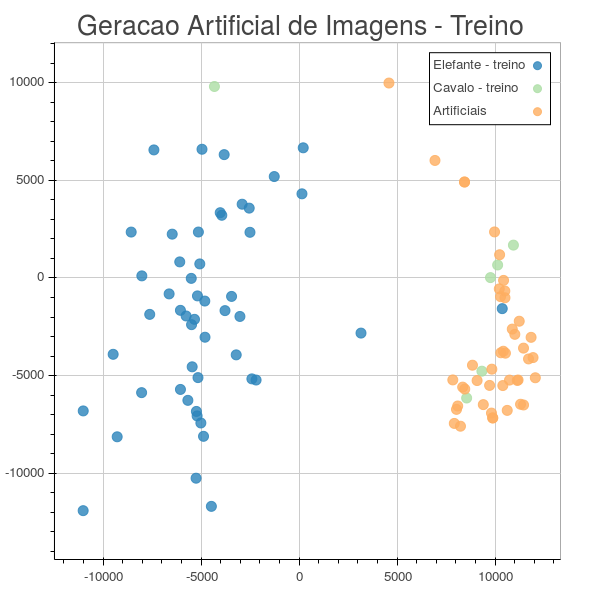
\includegraphics[width=\linewidth]{\detokenize{figuras/visualizacao/geracao-treino-fixed.png}}
    \end{subfigure}
  \end{center}
  \caption{Comparação dos examplos de treinamento da geração com SMOTE e no campo visual. Em laranja estão representados os novos exemplos, projetados no plano da base original balanceada.}
  \label{fig:compara_vis_treino_fixed}
\end{figure}

Após o treinamento realizado com as novas imagens e exemplos, o conjunto de teste foi fornecido ao classificador 1-NN e o resultado das predições está ilustrado na Figura~\ref{fig:compara_vis_teste}. A cor no interior dos marcadores quadrados representa a classe real dos exemplos e a borda representa a classe predita pelo classificador. Nota-se que a melhoria na classificação com a geração de imagens fica visível e corresponde ao aumento do \textit{f-score}.

\begin{figure}[htbp]
  \begin{center}
    \begin{subfigure}{.49\linewidth}
      \centering
      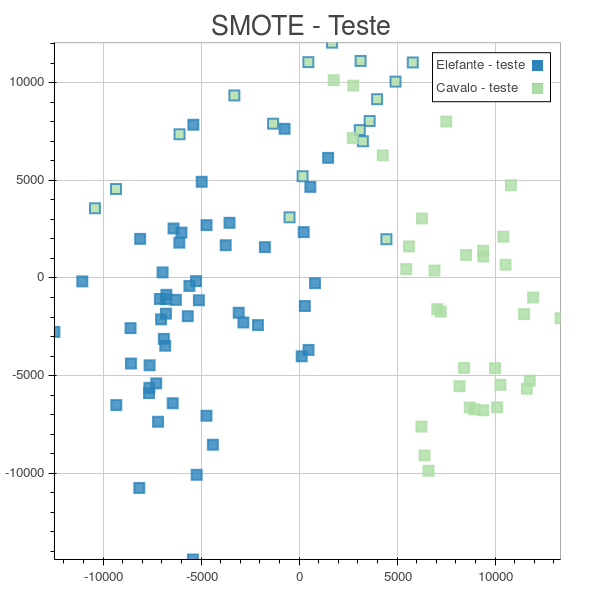
\includegraphics[width=\linewidth]{\detokenize{figuras/visualizacao/smote-teste-fixed.png}}
    \end{subfigure}
    \begin{subfigure}{.49\linewidth}
      \centering
      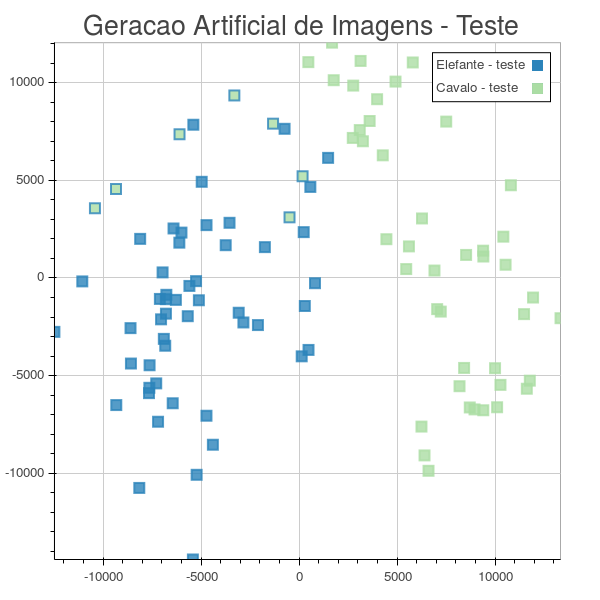
\includegraphics[width=\linewidth]{\detokenize{figuras/visualizacao/geracao-teste-fixed.png}}
    \end{subfigure}
  \end{center}
  \caption{Resultado do teste da classificação com 1-NN após o treinamento realizado com as bases rebalanceadas. A cor no interior dos marcadores quadrados representa a classe real dos exemplos e a borda representa a classe predita pelo classificador.}
  \label{fig:compara_vis_teste}
\end{figure}

De uma forma geral, pode-se dizer que a geração de imagens melhorou a definição da classe minoritária e foi o método que mais se assemelhou à distribuição dos dados originais. Além disso, um dos problemas do SMOTE pode ser verificado nessas projeções: ao realizar a interpolação dos vetores de características originais, pode-se criar exemplos em regiões do espaço que fazem parte da outra classe. Ficou claro também que o método SMOTE não possui capacidade de extrapolar a sua região, como pode ser observado no grupo de exemplos gerados à direita do espaço. O SMOTE gerou novos elementos em linha reta, enquanto a geração de imagens proporcionou uma abrangência maior em volta desse espaço, com maior dispersão.

É válido também visualizar a região de decisão, observando suas modificações frente aos métodos. Pode ser observado que em ambas técnicas a região da classe minoritária apresenta-se melhor representada. Além disso, é possível verificar que o SMOTE ocasionou uma certa ``invasão'' do espaço de características da classe majoritária.

\begin{figure}[htbp]
  \begin{center}
    \begin{subfigure}{.49\linewidth}
      \centering
      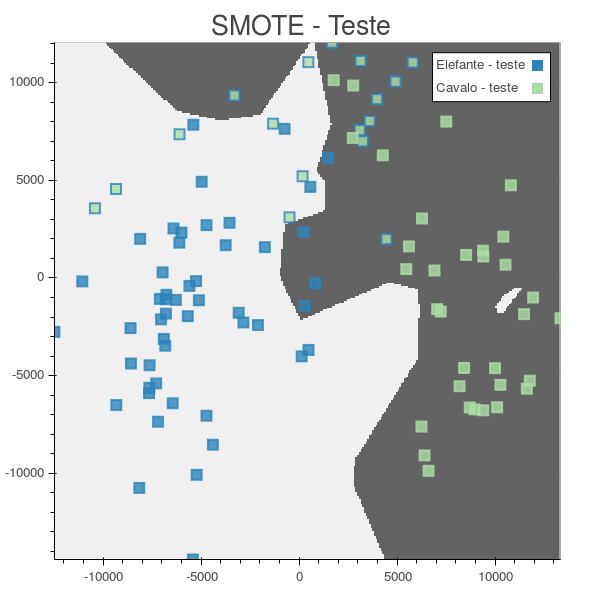
\includegraphics[width=\linewidth]{\detokenize{figuras/visualizacao/smote-teste-region.png}}
    \end{subfigure}
    \begin{subfigure}{.49\linewidth}
      \centering
      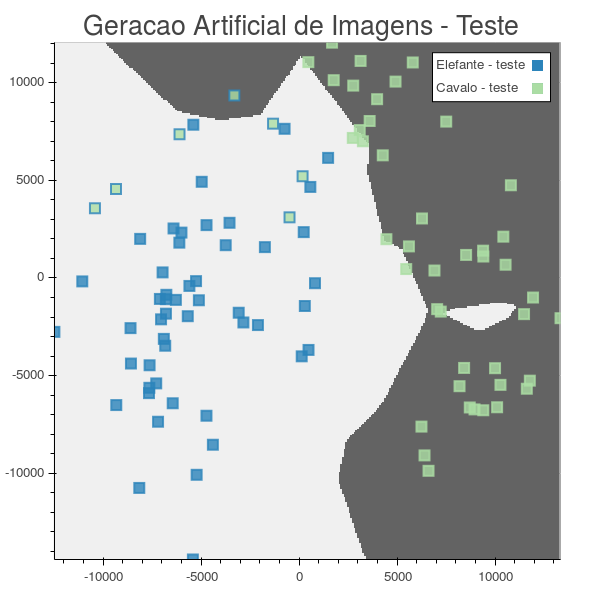
\includegraphics[width=\linewidth]{\detokenize{figuras/visualizacao/geracao-teste-region.png}}
    \end{subfigure}
    \begin{subfigure}{.49\linewidth}
      \centering
      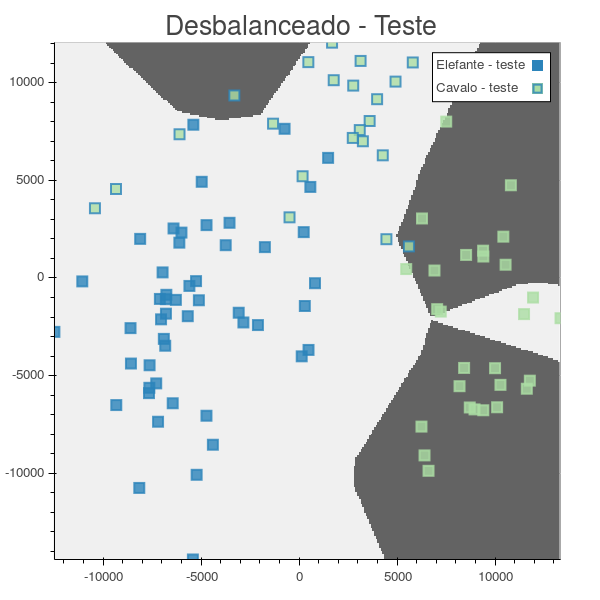
\includegraphics[width=\linewidth]{\detokenize{figuras/visualizacao/desbalanceado-teste-region.png}}
    \end{subfigure}
  \end{center}
  \caption{Região de decisão com K-NN (K = 1)}
  \label{fig:region}
\end{figure}

Nas figuras anteriores os exemplos foram projetados no plano criado pelas suas componentes principais com maior autovalores da base original balanceada. Se após a geração de novos exemplos essas componentes forem recalculadas (Figura \ref{fig:compara_vis_treino}), pode-se notar que a geração de imagens artificiais proporciona a criação de um subespaço que melhor discretiza as classes, quando comparado com SMOTE ou com a base desbalanceada.

\begin{figure}[htbp]
  \begin{center}
    \begin{subfigure}{.49\linewidth}
      \centering
      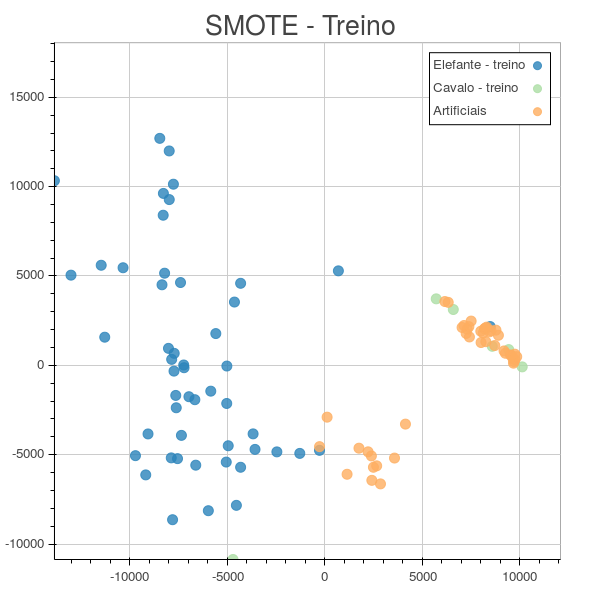
\includegraphics[width=\linewidth]{\detokenize{figuras/visualizacao/smote-treino.png}}
    \end{subfigure}
    \begin{subfigure}{.49\linewidth}
      \centering
      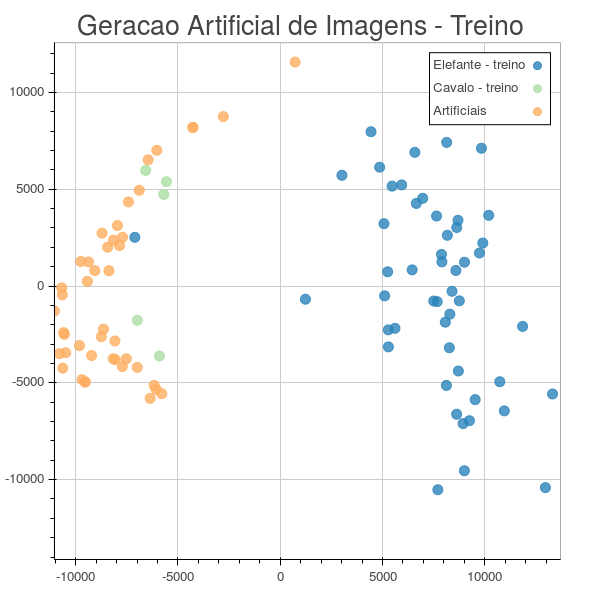
\includegraphics[width=\linewidth]{\detokenize{figuras/visualizacao/geracao-treino.png}}
    \end{subfigure}
    \begin{subfigure}{.49\linewidth}
      \centering
      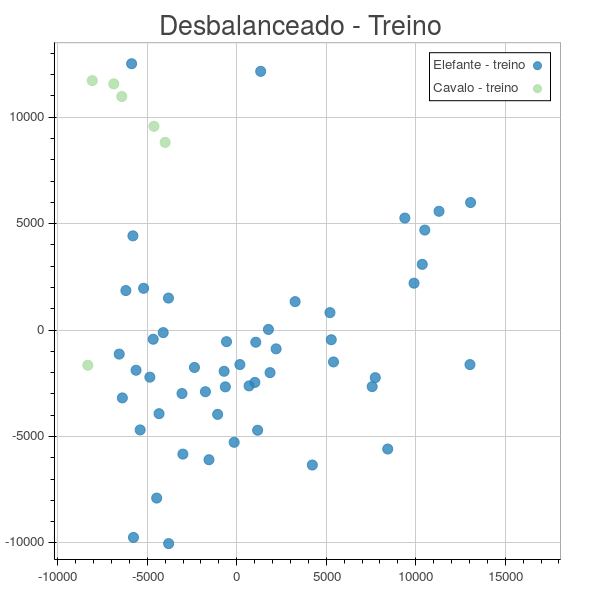
\includegraphics[width=\linewidth]{\detokenize{figuras/visualizacao/desbalanceado-treino.png}}
    \end{subfigure}
  \end{center}
  \caption{Melhores subespaços encontrados após a geração de novos exemplos para o SMOTE e para a geração artificial de imagens, e após a remoção de imagens para a projeção dos dados desbalanceados.}
  \label{fig:compara_vis_treino}
\end{figure}

Como relatado no início dessa seção, o extrator de características utilizado foi o BIC. Fundamentalmente ele captura informações de intensidade de cor das imagens. Na Figura~\ref{fig:vis_images} as próprias imagens foram utilizadas como marcadores na projeção do melhor subespaço após a geração artificial com o método de mistura. É nítido o impacto da etapa de extração de características na separação das classes e também no método de geração de imagens antes dessa extração.

\begin{figure}[htbp]
  \begin{center}
      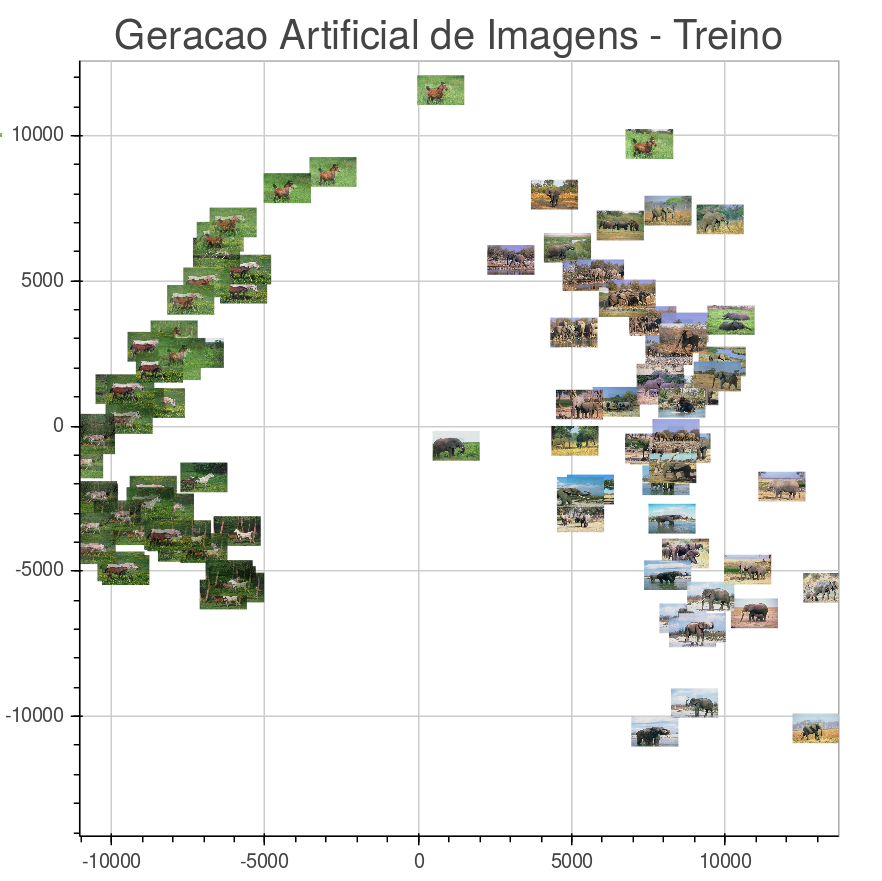
\includegraphics[width=\linewidth]{\detokenize{figuras/visualizacao/vis-images.png}}
  \end{center}
  \caption{Visualização do impacto do descritor de características.}
  \label{fig:vis_images}
\end{figure}

%--------------------------------------------------------------------------------
% \section{Considerações iniciais}
%
% Este capítulo apresenta os resultados preliminares obtidos. Primeiramente, é apresentada a descrição do experimento realizado, ressaltando os métodos de extração de características, quantização e classificação utilizados. Além disso, o fluxo de operações para a realização do experimento é descrito. Em seguida, os resultados são propriamente ilustrados, ao indicar que a geração de imagens artificiais é promissora para o cenário de bases desbalanceadas. Por fim, as atividades futuras são destacadas.
%
% %--------------------------------------------------------------------------------
% \section{Descrição do experimento}
%
% Algumas pesquisas sobre os efeitos da sobreamostragem e geração de exemplos artificiais em dados de aprendizado de máquina já foram realizadas~\cite{Kuncheva2004,Chawla2002}. O método mais divulgado na literatura é conhecido como SMOTE (\textit{Synthetic Minority Over-sampling Technique}). Este método propõe a geração de exemplos artificiais a partir dos vetores de características originais das classes minoritárias. Não há registro conhecido de um estudo dessas técnicas em dados de informação visual para o rebalanceamento de classes.
%
% % \enlargethispage{-\baselineskip}
%
% Assim, foi proposta a geração de novas imagens a partir de operações como adição de ruído, borramento, mistura e combinação das imagens originais. Tais operações estão exemplificadas na Figura~\ref{fig:ArtificialImages}, utilizando a classe ``praia'' da base de imagens naturais COREL-1000. A partir das imagens originais --- primeira linha da figura --- são geradas imagens artificiais por meio das operações citadas, resultando nas imagens da segunda linha da figura.
%
% \vspace{25pt}
%
% \renewcommand{\tabcolsep}{0.04cm}
% \begin{figure}[!h]
%  \begin{center}
%  \begin{tabular}{ccccc}
%    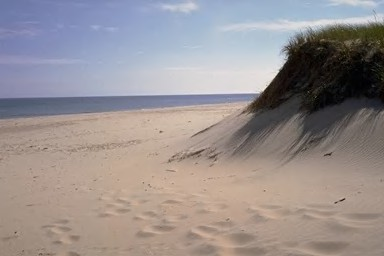
\includegraphics[width=0.245\linewidth]{\detokenize {figuras/original-1.jpg}}&
%    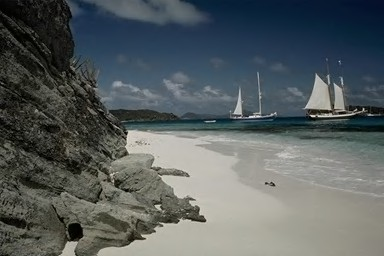
\includegraphics[width=0.245\linewidth]{\detokenize {figuras/original-2.jpg}}&
%    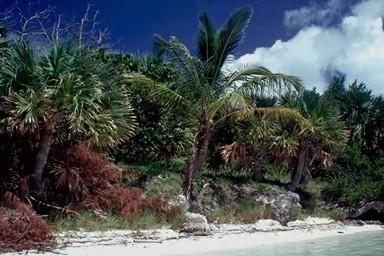
\includegraphics[width=0.245\linewidth]{\detokenize {figuras/original-3.jpg}}&
%    % 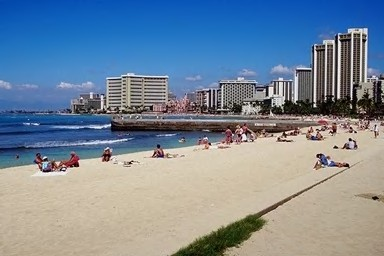
\includegraphics[width=0.19\linewidth]{\detokenize {figuras/original-4.jpg}}&
%    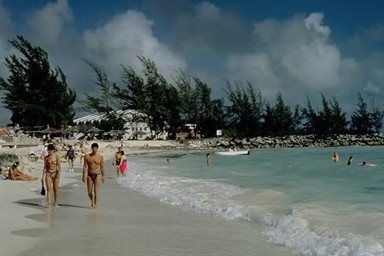
\includegraphics[width=0.245\linewidth]{\detokenize {figuras/original-5.jpg}}\\
%    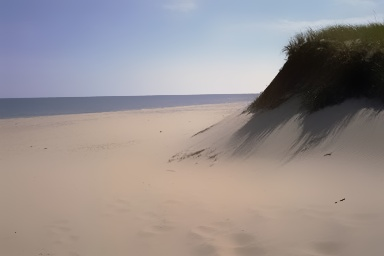
\includegraphics[width=0.245\linewidth]{\detokenize {figuras/gerada-1_blur.jpg}}&
%    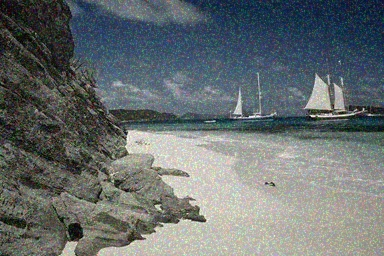
\includegraphics[width=0.245\linewidth]{\detokenize {figuras/gerada-2_ruido.jpg}}&
%    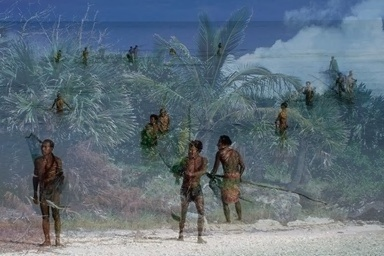
\includegraphics[width=0.245\linewidth]{\detokenize {figuras/gerada-3_blend.jpg}}&
%    % 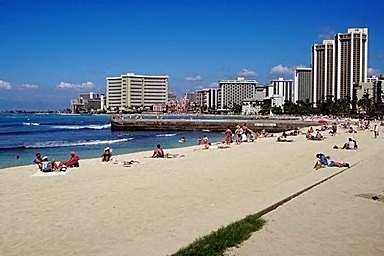
\includegraphics[width=0.19\linewidth]{\detokenize {figuras/gerada-4_unsharpMask.jpg}}&
%    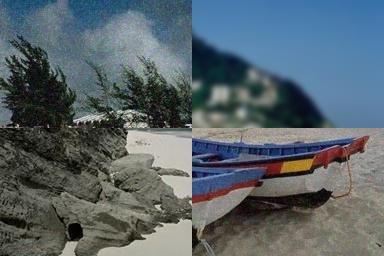
\includegraphics[width=0.245\linewidth]{\detokenize {figuras/gerada-5.jpg}} \\
%  \end{tabular}
%  \end{center}
%   \caption[Geração de imagens artificiais para o rebalanceamento de classes.]{Geração de imagens artificiais para o rebalanceamento de classes. A partir das imagens originais mostradas na primeira linha, são geradas imagens artificiais por meio de: borramento, adição de ruído, mistura e combinação. Os resultados dessas operações estão demonstrados na segunda linha, em ordem. \textit{Fonte:~Elaborado pela autora.}}
%  \label{fig:ArtificialImages}
% \end{figure}
% \renewcommand{\tabcolsep}{0.5cm}
% \vspace{25pt}
%
%
% Os descritores de características utilizados para os resultados foram apresentados na Seção \ref{sec:extracao}. \todo{qual experimento anterior? explicar!} Considerando que em um experimento anterior o melhor resultado foi atribuído à quantização com o método de Intensidade para o extrator Haralick e MSB para os outros, apenas esses testes foram aprofundados (tópico anteriormente discutido na Seção \ref{sec:quantizacao}). Neste experimento, o classificador KNN foi utilizado, com $K=1$. Inicialmente o classificador Naive Bayes foi explorado, apresentando melhora na acurácia ao apenas replicar as imagens. Esse comportamento não é desejado em um classificador para a avaliação de rebalanceamento de classes. O código desenvolvido para esses resultados preliminares está disponível em \url{https://bitbucket.org/moacirponti/imagefeatureextraction/overview}.
%
%
% %--------------------------------------------------------------------------------
% \subsection{Fluxo de operações}
%
% Para a realização desse experimento, iniciou-se com uma base originalmente balanceada e foram realizadas as seguintes operações:
%
% \begin{enumerate}
% \item Diminuir logaritmicamente o número de imagens de uma das classes, de modo a obter uma base desbalanceada;
% \item Para cada estágio de desbalanceamento, realizar três experimentos:
% \begin{enumerate}
% \item A classificação direta, sem nenhuma operação de rebalanceamento;
% \item A operação de SMOTE, após a extração de características e antes da classificação;
% \item Rebalanceamento da classe minoritária com a geração de imagens antes da extração de características.
% \label{item}
% \end{enumerate}
% \item Extrair as características com os descritores: ACC, BIC, CCV, GCH e Haralick6; e os quantizadores: Intensidade, Gleam, Luminância e MSB;
% \item Classificar com KNN utilizando validação cruzada por \textit{repeated random-subsampling};
% \item Executar os passos de 2 a 4 no mínimo 10 vezes para cada par de extrator e quantizador;
% \item Calcular a matriz de confusão, a acurácia balanceada, a medida-F e o teste de Friedman para os resultados encontrados;
% \item Gerar os gráficos para visualização dos resultados.
% \end{enumerate}
%
% %--------------------------------------------------------------------------------
% \subsection{Geração das imagens artificiais}
%
% As etapas para a geração das imagens artificiais, passo \ref{item} da seção anterior, foram:
%
% \begin{enumerate}
% \item Particionar a classe minoritária em conjuntos de treino e teste;
% \item Selecionar uma imagem aleatoriamente do conjunto de treino;
% \item Selecionar uma operação aleatória entre: borramento, adição de ruído, \textit{unsharp mask}, mistura ou composição;
% \begin{enumerate}
% \item Caso seja selecionada a composição: encontrar uma outra imagem aleatória, selecionar um quadrante dessa imagem e novamente uma operação entre: borramento, adição de ruído, \textit{unsharp mask} ou mistura;
% \end{enumerate}
% \item Aplicar essa operação na imagem previamente selecionada e adicionar essa imagem gerada ao conjunto de treino;
% \item Repetir os passos 2 a 4 até que as classes estejam igualmente balanceadas.
% \end{enumerate}
%
% %--------------------------------------------------------------------------------
% \section{Resultados}
% \label{sec:resultadospreliminares}
%
% Este estudo preliminar apresentou evidências experimentais de que, em problemas de duas classes (apresentadas na Figura~\ref{fig:praiamontanha}), pode haver ganho estatístico da medida-F ao gerar imagens, quando comparado à geração de exemplos artificiais no espaço de atributos (ou seja, depois que as características já foram extraídas das imagens). Essa melhoria pode ser notada na Figura~\ref{fig:resultmelhor}, que apresenta a relação da medida-F com a taxa de balanceamento, utilizando: as imagens originais, a geração de exemplos com SMOTE e as imagens geradas. Para essa configuração, foi utilizado o descritor de características ACC com a conversão em escala de cinza por MSB e a operação de pré-processamento por combinação. As classes ``praia'' e ``montanha'' foram escolhidas por serem as classes que possuem maior dificultade de diferenciação, havendo alta taxa de sobreposição de intensidades de cores e texturas, conforme testes realizados.
%
% \vspace{20pt}
%
% \begin{figure}[!htb]
%  \begin{center}
%    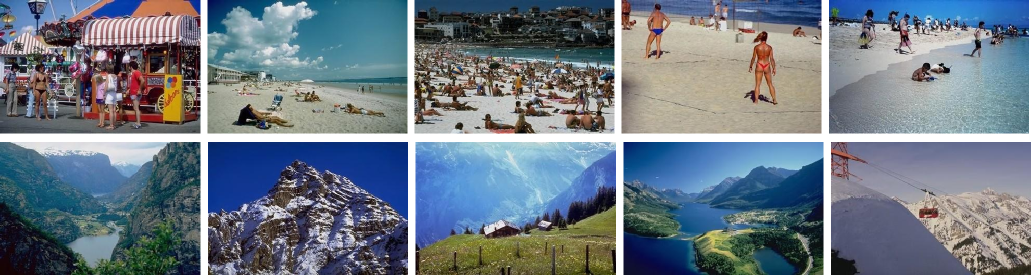
\includegraphics[width=\linewidth]{\detokenize {figuras/praia-montanha.png}}
%  \end{center}
%   \caption[Classes ``praia'' e ``montanha'' da base de imagens COREL-1000.]{Classes ``praia'' (primeira linha) e ``montanha'' (segunda linha) da base de imagens COREL-1000. \textit{Fonte:~Elaborado pela autora.}}
%  \label{fig:praiamontanha}
% \end{figure}
%
% \vspace{10pt}
%
% \begin{figure}[!hbpt]
%  \begin{center}
% \begin{subfigure}{\textwidth}
%   \centering
%   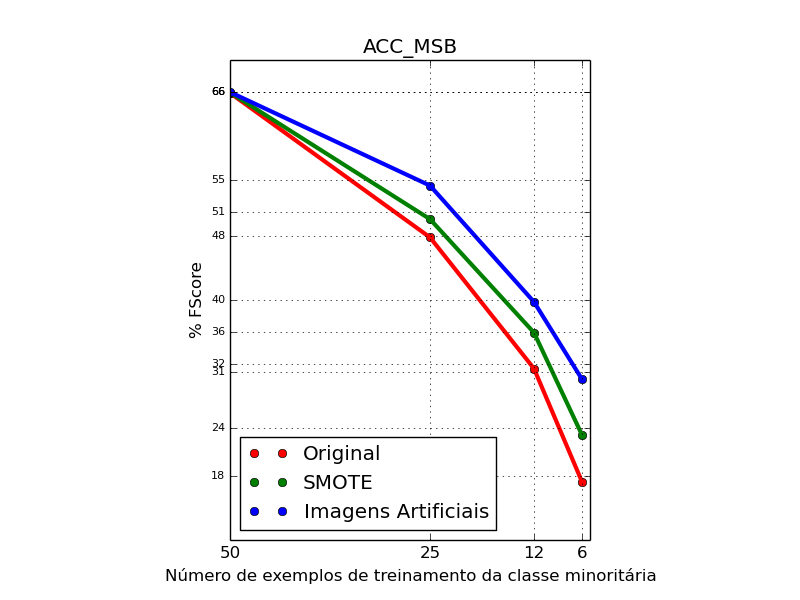
\includegraphics[width=\linewidth]{\detokenize {figuras/resultado-melhor4.png}}
%   \caption{Original}
% \end{subfigure}
% \begin{subfigure}{\textwidth}
%   \centering
%   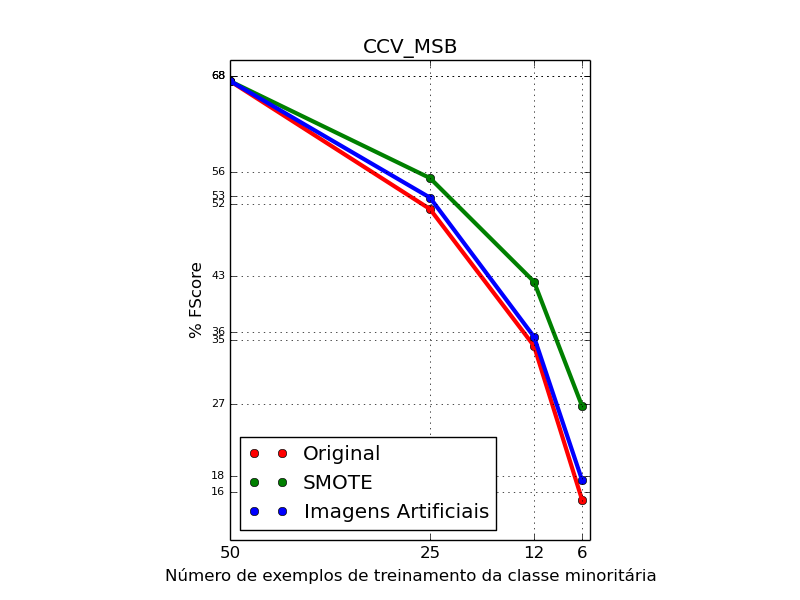
\includegraphics[width=\linewidth]{\detokenize {figuras/resultado-pior1.png}}
%   \caption{\textit{Unsharp masking}}
%   \label{fig:unsharp}
% \end{subfigure}
%  \end{center}
% \end{figure}
%
% \begin{figure}[htb]
%  \begin{center}
%    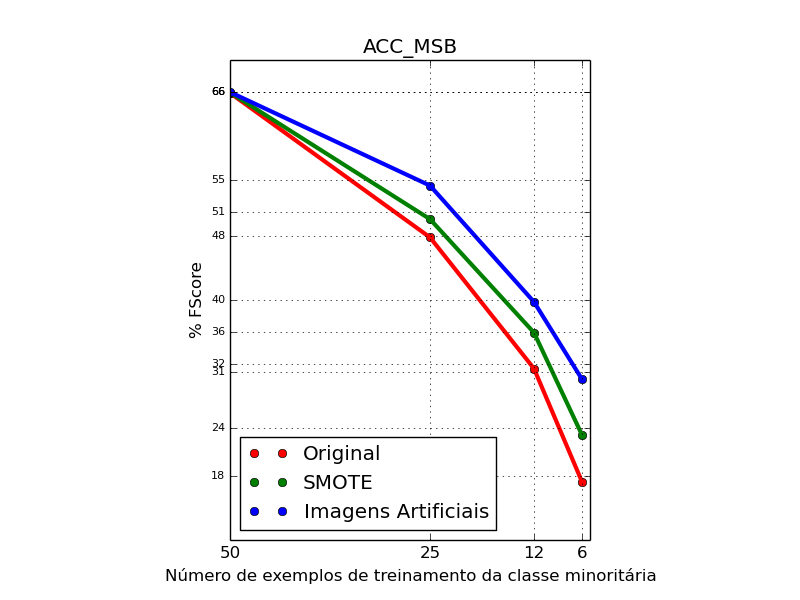
\includegraphics[width=\linewidth]{\detokenize {figuras/resultado-melhor4.png}}
%  \end{center}
%  \caption[Resultado obtido com a operação de combinação apresentada na Figura~\ref{fig:ArtificialImages}.]{Resultado obtido com a operação de combinação apresentada na Figura~\ref{fig:ArtificialImages}. Apresenta-se a relação da medida-F com a taxa de balanceamento utilizando: as imagens originais, a geração de exemplos com SMOTE e as imagens geradas artificialmente. \textit{Fonte:~Elaborado pela autora.}}
%  \label{fig:resultmelhor}
% \end{figure}
%
% \enlargethispage{-1cm}
%
% Também foi possível notar que algumas operações não provocaram a melhora da classificação. A operação de adição de ruído para geração artificial, a posterior extração utilizando CCV e a quantização por MSB, destacou-se como o pior resultado, apresentado na Figura~\ref{fig:resultpior}. Outros casos que não obtiveram o resultado esperado envolveram as operações de borramento e de \textit{unsharp masking}.
%
% \begin{figure}[htb]
%  \begin{center}
%    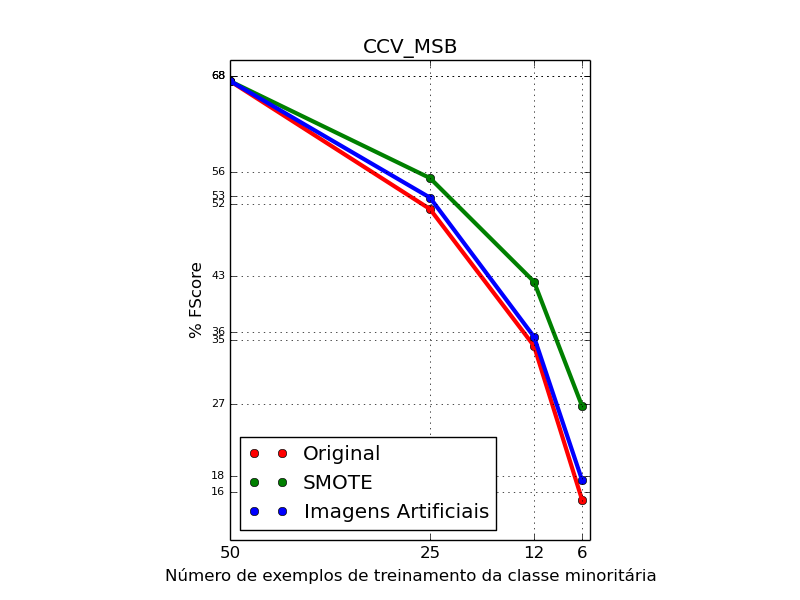
\includegraphics[width=\linewidth]{\detokenize {figuras/resultado-pior1.png}}
%  \end{center}
%  \caption[Piores resultados, obtidos com a adição de ruído.]{Piores resultados, obtidos com a adição de ruído. Apresenta-se a relação da medida-F com a taxa de balanceamento utilizando as imagens originais, o SMOTE e as imagens artificiais geradas. \textit{Fonte:~Elaborado pela autora.}}
%  \label{fig:resultpior}
% \end{figure}
%
% Após a realização dos testes, as operações que melhor se destacaram foram: utilizar todas as operações, apenas mistura e apenas composição. E as operações que resultaram em uma classificação pior do que o uso do SMOTE foram: utilizar apenas borramento, ruído ou \textit{unsharp masking}. Com o teste estatístico de Friedman foi possível verificar que o ACC foi o extrator que melhor se beneficiou das características geradas; e CCV e GCH os menos beneficiados. \enlargethispage{-\baselineskip} A Tabela \ref{tab:result} apresenta os \textit{rankings} encontrados por este teste para todas as execuções das melhores operações. O p-valor computado corresponde a $4.24E^{-11}$, assim a hipótese nula de que não há diferença entre as execuções foi rejeitada. Vale destacar que para algumas execuções, o teste de Friedman retornou o \textit{ranking}: geração artificial (1), SMOTE (2) e imagens originais (3), ou seja, sem que SMOTE e a geração artificial concorressem pela mesma posição, diferente da tabela apresentada.
%
% \begin{table}[htb]
% \centering
% \caption{Posição média dos algoritmos utilizando Friedman}
%   \begin{tabular}{c|c}
%     Algoritmos  &   Posição \\ \hline
%     Original    &   3.0000  \\
%     Smote       &   1.6136  \\
%     Artificial  &   1.3863  \\
%   \end{tabular}
%  \label{tab:result}
% \end{table}
%
% Em outro experimento, utilizou-se as cópias das imagens de treino para rebalancear, sem realizar nenhuma operação de pré-processamento (método conhecido como SRS - \textit{Simple Random Sampling}). A Figura~\ref{fig:resultcopia} mostra as respectivas medidas-F encontradas. É possível notar que a cópia dessas imagens não adiciona nenhuma informação nova para o aprendizado.
%
% \begin{figure}[htb]
%  \begin{center}
%    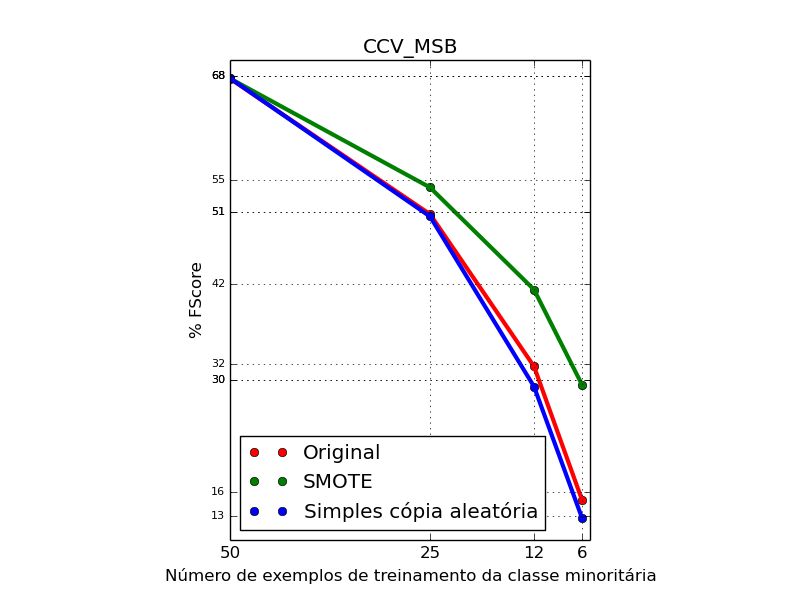
\includegraphics[width=\linewidth]{\detokenize {figuras/resultado-copia.png}}
%  \end{center}
%   \caption[Simples replicação de exemplos sem realizar nenhuma operação.]{Simples replicação de exemplos sem realizar nenhuma operação de pré-processamento. É possível verificar que não foi adicionada nenhuma informação relevante para o aprendizado. \textit{Fonte:~Elaborado pela autora.}}
%  \label{fig:resultcopia}
% \end{figure}
%
%
\section{Considerações Finais}

% Com os experimentos realizados foi possível notar que a geração de imagens artificiais pode gerar novas informações para a classificação das imagens. O que indica que um estudo mais aprofundado de quais operações podem ser aplicadas nas imagens originais auxilie o cenário de bases desbalanceadas.
%
% Dessa forma, esse capítulo também apresentou as próximas tarefas a serem realizadas. Foi destacada a análise das redes de convolução para identificar quais características latentes são automaticamente extraídas. Apesar de algumas operações de pré-processamento terem gerado imagens que melhoraram a classificação, algumas não causaram melhora. Isso indica que a análise da relevância da informação contida em imagens deve melhorar esse resultado. A memória associativa, aprendida com uma máquina de Boltzmann restrita, deve ser capaz de indicar se uma determinada imagem é relevante para o aprendizado.
